% Slides for 2024-07-02
% To create a slide, use the following:

\begin{frame}{OVERVIEW}

   Training AI models to detect and track Nassau grouper in videos
\end{frame}


\begin{frame}{OVERVIEW}
    \centering
     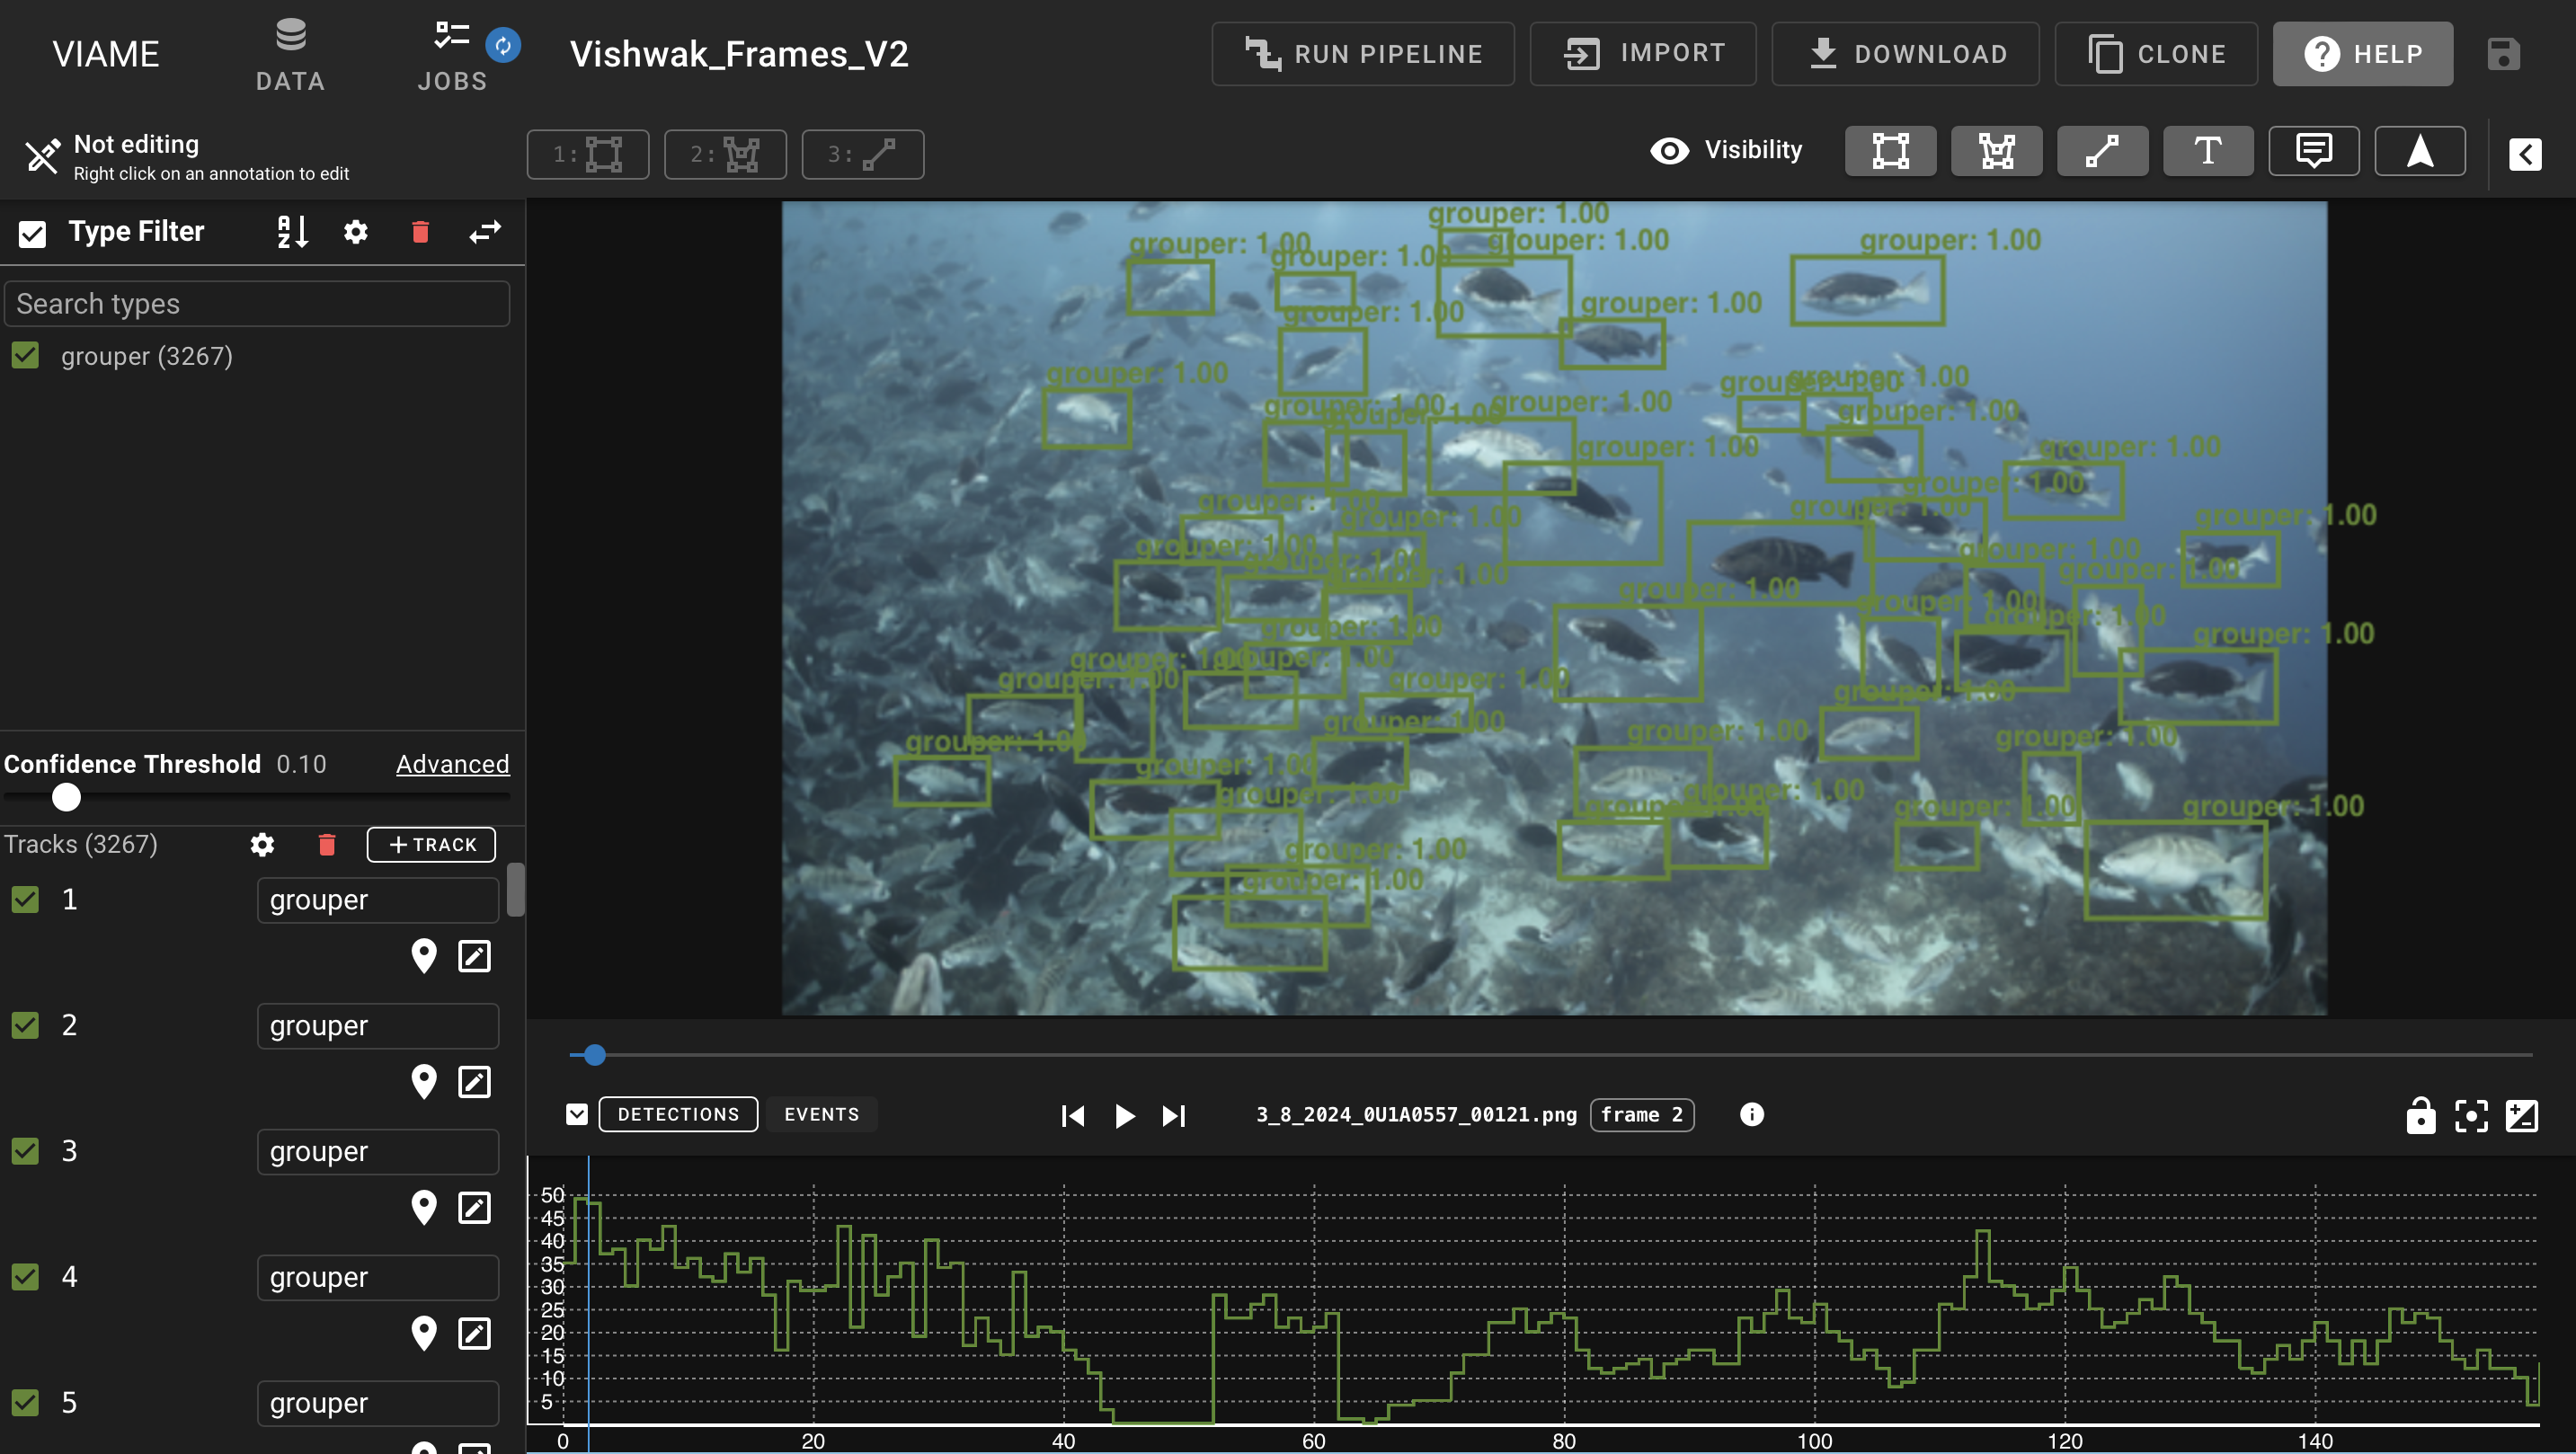
\includegraphics[height=0.7\textheight,width=0.7\textwidth,keepaspectratio]{gm1.png}
     
\end{frame}

\begin{frame}{TASKS}
    \begin{itemize}
        \item Training detection model on VIAME
        \item Training tracker on VIAME 
        \item Developing an algorithm which automates image selection to be representative of the fish being tracked
        \item Use the selected image for pattern recognition (give each fish an id)
    \end{itemize}
\end{frame}

% To create a slide with a bullet list, use the following:
% \begin{frame}{TITLE}
%     \begin{itemize}
%         \item ITEM 1
%         \item ITEM 2
%     \end{itemize}    
% \end{frame}

% To create a slide with numbered list, use the following:
% \begin{frame}{TITLE}
%     \begin{enumerate}
%         \item ITEM 1
%         \item ITEM 2
%     \end{enumerate}
% \end{frame}

% To create a slide with a graphic:
% 1. Add the graphic to this folder (named picture.png)
% 2. Use the following:
% \begin{frame}{TITLE}
%     \centering
%     \includegraphics[height=0.7\textheight,width=0.7\textwidth,keepaspectratio]{picture.png}
% \end{frame}

% To create a slide with two columns, use the following:
% \begin{frame}{TITLE}
%     \begin{columns}
%         \begin{column}{0.5\textwidth}
%             COLUMN 1 BODY
%         \end{column}
%         \begin{column}{0.5\textwidth}
%             COLUMN 2 BODY
%         \end{column}
%     \end{columns}
% \end{frame}
